%%=============================================================================
%% Methodologie
%%=============================================================================

\chapter{\IfLanguageName{dutch}{Methodologie}{Methodology}}%
\label{ch:methodologie}

%% TODO: In dit hoofstuk geef je een korte toelichting over hoe je te werk bent
%% gegaan. Verdeel je onderzoek in grote fasen, en licht in elke fase toe wat
%% de doelstelling was, welke deliverables daar uit gekomen zijn, en welke
%% onderzoeksmethoden je daarbij toegepast hebt. Verantwoord waarom je
%% op deze manier te werk gegaan bent.
%% 
%% Voorbeelden van zulke fasen zijn: literatuurstudie, opstellen van een
%% requirements-analyse, opstellen long-list (bij vergelijkende studie),
%% selectie van geschikte tools (bij vergelijkende studie, "short-list"),
%% opzetten testopstelling/PoC, uitvoeren testen en verzamelen
%% van resultaten, analyse van resultaten, ...
%%
%% !!!!! LET OP !!!!!
%%
%% Het is uitdrukkelijk NIET de bedoeling dat je het grootste deel van de corpus
%% van je bachelorproef in dit hoofstuk verwerkt! Dit hoofdstuk is eerder een
%% kort overzicht van je plan van aanpak.
%%
%% Maak voor elke fase (behalve het literatuuronderzoek) een NIEUW HOOFDSTUK aan
%% en geef het een gepaste titel.

The research will be divided into 6 phases, the first of which is a literature review. Literature research will be performed to examine existing approaches, explore popular languages, and gain a deeper understanding of the state of the art. The result of this literature search can be found in section 2 of this research proposal.

Phase 2 consists of creating a list of minimal requirements for a suitable language choice. Possible types of requirements could include ease of use, security implications, performance, and suitability for IAM-related tasks. A concrete list of measurable requirements will be assembled in consultation with thesis stakeholders and employees at TrustBuilder. The MoSCoW method will be used to order these requirements by importance, and each requirement will be marked as functional or non-functional.

Phase 3 is to create a long list of options, checked against the previously listed requirements. The literature review from phase 1 will be used to build an exhaustive list of suitable language choices. Popular existing options, as well as possibly lesser-known choices, will be considered.

Phase 4 aims to create a short list of the three most promising options, using a requirements summary table.

In phase 5, a proof of concept will be created to validate the suitability of each language in the short list. The proof of concept will consist of a simple HTTP server for each chosen language, which will allow running code that handles HTTP requests in the specified language. Three scripts will be written for each language, and will handle three distinct needs. The exact functionality of these three types of scripts will be decided based on TrustBuilder's typical customization requirements. This proof of concept will help further solidify and compare each language's suitability for customizing and extending IAM systems, and will provide deeper insight in their tooling and ease of use for these purposes.

Phase 6 will consist of drawing conclusions out of the research and propose next steps. The results and findings from the previous phases will be analyzed, and limitations and areas for future research will be identified.

Throughout this entire process, a thesis will be written that documents the research, findings, and proposed solutions.

\begin{figure}[h]
    \centering
    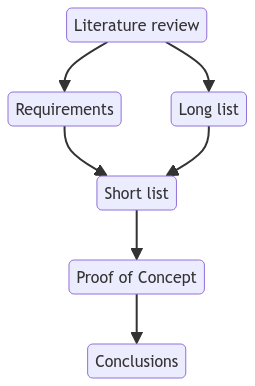
\includegraphics[height=.3\paperheight]{methodology.png}
    \caption{A flowchart representation of the methodology}
\end{figure}
